%\documentclass[spanish]{beamer}

\documentclass{beamer}
\usepackage{pgf,pgfpages}
%\pgfpagesuselayout{4 on 1}[letterpaper,landscape,border shrink=0.5in]
\usepackage{algorithm,algorithmic}
%\usepackage{algorithm,algorithmicx}
%\usepackage[noend]{algpseudocode}
\usepackage{listings}
\lstset{basicstyle=\ttfamily,
	showstringspaces=false,
	commentstyle=\color{red},
	literate={á}{{\'a}}1
	{ã}{{\~a}}1
	{é}{{\'e}}1
	{ó}{{\'o}}1
	{í}{{\'i}}1
	{ñ}{{\~n}}1
	{¡}{{!`}}1
	{¿}{{?`}}1
	{ú}{{\'u}}1
	{Í}{{\'I}}1
	{Ó}{{\'O}}1
}

\usepackage{beamerthemesplit}
\usepackage{color}
\usepackage[utf8]{inputenc}
\usepackage[spanish]{babel}
%\usepackage[latin1]{inputenc}
%\usepackage[pdftex]{graphicx}
%\usepackage{algorithm}
%\usepackage{algorithmic-C}
%\usepackage{algorithmic}
\usepackage{amsthm}
\usepackage{multicol}
\usepackage{multirow}
\usepackage{fancyvrb,relsize}
\usepackage{hhline}
\usepackage{tikz}
\usetikzlibrary{trees, shapes, calc}
\newcommand{\inputTikZ}[2]{%
	\scalebox{#1}{\input{#2}}
}

\usetheme{Warsaw} %Gueno
%\usetheme{Darmstadt} %OK!
% \usetheme{Frankfurt} %OK!
%\usetheme{Goettingen}
%\usetheme{Dresden}
%\usetheme{JuanLesPins} %OK!!
%\usetheme{Marburg}
%\usetheme{Montpellier}
%\usetheme{Rochester} %sobrio
%\usetheme{Singapore}
%\usetheme{Szeged}

%\usecolortheme{albatross}
%\usecolortheme{seahorse}
%\usecolortheme{beetle}
%\usecolortheme{crane}
%\usecolortheme{dolphin}
%\usecolortheme{dove}
%\usecolortheme{fly}
%\usecolortheme{lily} %Gueno
\usecolortheme{orchid}%Gueno
%\usecolortheme{rose}
%\usecolortheme{seagull}
%\usecolortheme{whale}


\DefineVerbatimEnvironment%
      {VerbatimNN}%
      {Verbatim}%
      {fontsize=\relsize{-1}}
\DefineVerbatimEnvironment%
      {VerbatimNNN}%
      {Verbatim}%
      {fontsize=\relsize{-2}}

\DefineVerbatimEnvironment%
      {VerbatimPseudo}%
      {Verbatim}%
      {numbers=left, fontsize=\relsize{-1}}
\DefineVerbatimEnvironment%
      {VerbatimPseudoReduced}%
      {Verbatim}%
      {numbers=left, fontsize=\relsize{-2}}
\DefineVerbatimEnvironment%
      {VerbatimPseudoReduced2}%
      {Verbatim}%
      {numbers=left, fontsize=\relsize{-3}}
\DefineVerbatimEnvironment%
      {VerbatimC}%
      {Verbatim}%
      {commandchars=@ªº, numbers=left, fontsize=\relsize{-1}}
\DefineVerbatimEnvironment%
      {VerbatimReducedC}%
      {Verbatim}%
      {commandchars=@ªº, numbers=left, fontsize=\relsize{-2}}
\DefineVerbatimEnvironment%
      {VerbatimReduced2C}%
      {Verbatim}%
      {commandchars=@ªº, numbers=left, fontsize=\relsize{-3}}



%\AtBeginSubsection[]
%{
% \begin{frame}
% \frametitle{Sinopsis}
% Aqui decides: cada seccion y subseccion:
% \tableofcontents[currentsection,currentsubsection]
 %O solamente la seccion (Solo uno de ellos)
%\tableofcontents[currentsection]
% \end{frame}
%}

% Si quieres que todo por default aparezca de poco en poco
% descomenta esta linea
%\beamerdefaultoverlayspecification{<+->}

\setbeamertemplate{footline}{\hfill\insertframenumber/\inserttotalframenumber}
\setbeamertemplate{navigation symbols}{}

\setbeamercovered{transparent}

\title{ELO320 - Estructuras de Datos y Algoritmos\\Introducción a C\\Hello World!}
%\subtitle{Ingeniería Civil Telemática UTFSM}
\author{Dr. Nicolás Gálvez R.\\{\small nicolas.galvez@usm.cl}}
\institute{Ing. Civil Telemática - Departamento de Electrónica}
\titlegraphic{
\includegraphics[scale=.125]{images/logoutfsm}}
\date{1er Semestre 2025}

\begin{document}

\frame{\titlepage}

%\section*{Sinopsis}
%\frame{  \frametitle{Sinopsis}\tableofcontents[pausesections]}
%
%

\section{¿Por qué C?}

\begin{frame}{Programación Estructurada}
	\begin{block}{}
		{\small\textbf{Paradigma de programación} basado en el \textbf{uso extensivo de subrutinas y estructuras de control}, con el fin de mejorar la \textbf{claridad}, \textbf{calidad} y \textbf{tiempo de desarrollo} del código de programas computacionales.}
	\end{block}
	\begin{itemize}
		\item \textbf{C, lanzado en 1973, es el mayor exponente de este tipo de lenguajes.}
	\end{itemize}
	\vspace{-.25cm}
	\begin{center}
		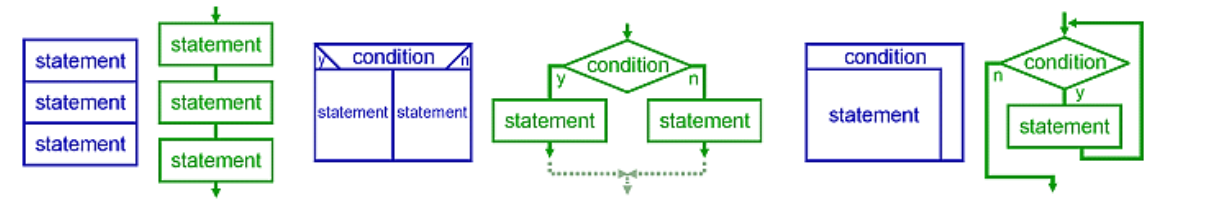
\includegraphics[width=\linewidth]{images/structured.png}
	\end{center}
\end{frame}

\begin{frame}{¿Por qué es C tan relevante?}
\begin{itemize}
\item Diseñado para desarrollar UNIX OS.
\item Maneja actividades de bajo nivel (en la memoria), a pesar de ser un lenguaje de alto nivel.
\item Se relaciona eficientemente con instrucciones de máquina.
\item Perdura su uso en el tiempo.
\item La mayoría de software tiene una relación directa o indirecta con C.
\end{itemize} 
\end{frame}

\section{Elementos Generales}
\begin{frame}[fragile]{Elementos Generales - Datos}
\begin{itemize}
	\footnotesize
	\item \textbf{Datos Primitivos:} enteros, reales, caracteres.
	\vspace{-.45cm}
	\begin{columns}[t]
		\begin{column}{5.1cm}
		\begin{exampleblock}{C}
		\begin{lstlisting}[language=C,basicstyle=\scriptsize]
int contador = 10;
char nombre[10] = "Eduardo";
float PI = 3.14159;
		\end{lstlisting}
		\end{exampleblock}
		\end{column}
		\begin{column}{5.1cm}
		\begin{block}{Python}
		\begin{lstlisting}[language=Python, basicstyle=\scriptsize]
contador = 10
nombre = "Eduardo"
PI = 3.14159
		\end{lstlisting}
		\end{block}
		\end{column}
	\end{columns}
	\vspace{.15cm}
	\item \textbf{Estructurados:} agrupar/componer conjuntos de datos del mismo tipo en una unidad (e.g. Arreglo). 
	\vspace{-.45cm}
	\begin{columns}[t]
		\begin{column}{5.1cm}
		\begin{exampleblock}{C}
		\begin{lstlisting}[language=C,basicstyle=\scriptsize, escapeinside={|}{|}]
char semana[5][20] =
{"Lu","Ma","Mi","Ju","Vi"};
printf("|\%s|\n", semana[1]);
		\end{lstlisting}
		\end{exampleblock}
		\end{column}
		\begin{column}{5.1cm}
		\begin{block}{Python}
		\begin{lstlisting}[language=Python,basicstyle=\scriptsize]
semana = ["Lu","Ma","Mi",
          "Ju","Vi"]
print(semana[1])
		\end{lstlisting}
		\end{block}
		\end{column}
	\end{columns}
	\vspace{.15cm}
\end{itemize}
\end{frame}

\begin{frame}[fragile]{Elementos Generales - Estructuras de Control}
\small
\vspace{-.25cm}
	\begin{itemize}
		\footnotesize
		\item \textbf{Sentencias:} abstrae conjunto de instrucciones.
		\item \textbf{Estructuras de control:} secuenciación, condición y repetición (e.g. if, while).
		\item \textbf{Abstracción procedural:} procedimiento con un nombre y parámetros (e.g. funciones y métodos).
		\item \textbf{Concurrencia:} computación paralela (e.g. procesos y hebras). 
	\end{itemize}
	\small
\end{frame}

\begin{frame}[fragile]{Métodos de Implantación}
\begin{itemize}
	\item \textbf{Compilación:} (e.g. C, C++)\\
	Traduce a lenguaje de máquina para posterior ejecución (interpretación directa por el procesador).
	\item \textbf{Interpretación:} (e.g. LISP, Python)\\
	Una máquina virtual interpreta directamente el código fuente durante la ejecución.
	\item \textbf{Híbrido:} (e.g. Java, C\#)\\
	Se compila a un lenguaje intermedio, que luego es interpretado.
\end{itemize}
\end{frame}

\begin{frame}[fragile]{Uso de Código en C}
\large
\begin{itemize}
	\item \textbf{Modularización:} descomponer programas en unidades de desarrollo más pequeñas (módulos). 
	\item \textbf{Compilación Separada o Indepediente:} Módulos de un programa se pueden compilar por separado (bibliotecas).
	\item \textbf{Reutilización:} Módulos y clases se pueden reutilizar para diferentes programas. 
\end{itemize}
\end{frame}

\begin{frame}[fragile]{Popularidad de Lenguajes (stackoverflow, redmonk)}
\vspace{-.25cm}
\begin{center}
	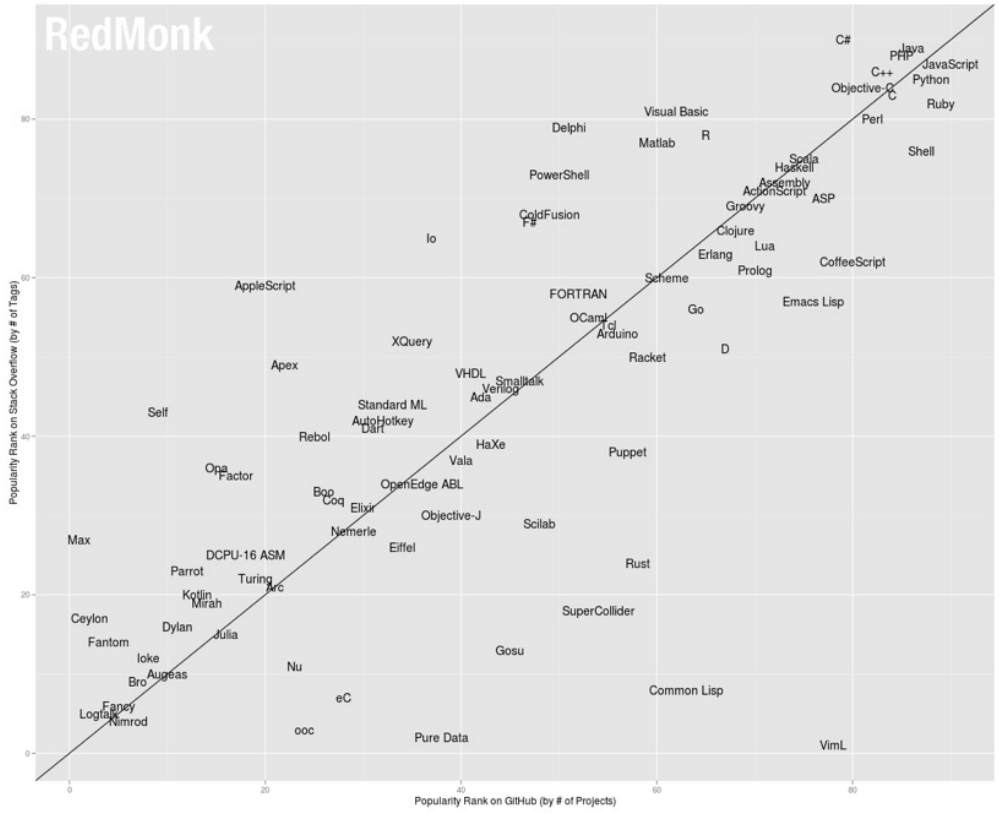
\includegraphics[width=.8\linewidth]{images/01-popularity.png}
\end{center}
\end{frame}

\begin{frame}[fragile]{Rendimiento de Lenguajes}
\begin{center}
	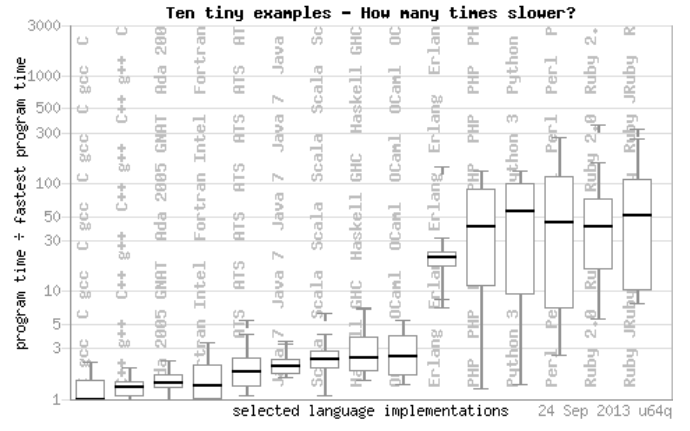
\includegraphics[width=.7\linewidth]{images/01-benchmark.png}
\end{center}

%\Large
\url{http://benchmarksgame.alioth.debian.org/u32/performance.php}
\end{frame}

\section{Aprendamos C}

\subsection{Estructura General}
\begin{frame}[fragile]{C Estructura general}
\begin{itemize}
	\item Requiere un método de inicio de ejecución: \textbf{main}
\end{itemize}

%\vspace{-.45cm}
%  \begin{columns}[t]
%\begin{column}{5.1cm}
\begin{exampleblock}{C}
\begin{lstlisting}[language=C,basicstyle=\scriptsize]
#include<stdio.h>

int main() {
	printf("Hola Mundo\n");
	return 0;
}
\end{lstlisting}
\end{exampleblock}
%\end{column}
%\begin{column}{5.1cm}
\begin{block}{Python}
	\begin{lstlisting}[language=Python,basicstyle=\scriptsize]
if __name__ == "__main__":
	print("Hola Mundo!")
	\end{lstlisting}
\end{block}
%\end{column}
%\end{columns}
\end{frame}

\end{document}
